\section{Resoconto attività di verifica}
In questa sezione sono descritte le attività di verifica svolte sui documenti che vengono presentati alle revisioni di avanzamento. Qualora una verifica riscontrasse un problema su un documento, nella sezione \S B si discuterà di quali siano i possibili miglioramenti, anche in relazione ad un piano di incremento continuo (PDCA).
Inoltre verranno utlizzate delle sigle per fare riferimento al periodo in cui sono stati rilevati i risultati delle verifiche. Le sigle sono le seguenti:
\begin{itemize}
\item \textbf{An}: Analisi;
\item \textbf{TB}: Technology Baseline;
\item \textbf{PB}: Product Baseline;
\item \textbf{VC}: Validazione e Collaudo. 
\end{itemize}

\subsection{Analisi dei documenti}
\subsubsection{Analisi statica}
L'analisi dei documenti mediante Walkthrough (vedi \textit{Norme di Progetto}) ha portato all'individuazione di alcuni errori frequenti a partire dai quali è stata stilata una check list. In questo modo sarà possibile applicare l’Inspection (vedi \textit{Norme di Progetto}) per le future attività di verifica.


\paragraph{Esiti MD01 - Indice di Gulpease} \mbox{} \\
\begin{longtable}{c c c c c c}
\rowcolor{white}\caption{Esiti MD01 - Indice di Gulpease} \\
		\rowcolor{redafk}
\textcolor{white}{\textbf{Documento}} &
\textcolor{white}{\textbf{An}} &
\textcolor{white}{\textbf{TB}} &
\textcolor{white}{\textbf{PB}} &
\textcolor{white}{\textbf{VC}} &
\textcolor{white}{\textbf{Esito}} \\
		\endfirsthead
		\rowcolor{white}\caption[]{(continua)} \\
		\rowcolor{redafk}
\textcolor{white}{\textbf{Documento}} &
\textcolor{white}{\textbf{An}} &
\textcolor{white}{\textbf{TB}} &
\textcolor{white}{\textbf{PB}} &
\textcolor{white}{\textbf{VC}} &
\textcolor{white}{\textbf{Esito}} \\
		\endhead
		\textit{Analisi dei Requisiti} & 70 & 73 & 74 & 74 & Ottimale \\
		\textit{Glossario} & 74 & 74 & 74 & 74 & Ottimale \\
		\textit{Norme di Progetto} & 67 & 70 & 72 & 72 & Ottimale \\
		\textit{Piano di Progetto} & 72 & 71 & 73 & 75 & Ottimale \\
		\textit{Piano di Qualifica} & 69 & 72 & 71 & 71 & Ottimale \\
		\textit{Studio di Fattibilità} & 70 & - & - & - & Ottimale \\
		\textit{Media Verbali} & 71 & 74 & 76 & 80 & Ottimale\\
		\textit{Manuale Utente} & - & - & 65 & 66 & Ottimale \\
		\textit{Manuale Sviluppatore} & - & - & 68 & 68 & Ottimale \\
\end{longtable}

\begin{figure}[H]
\centering
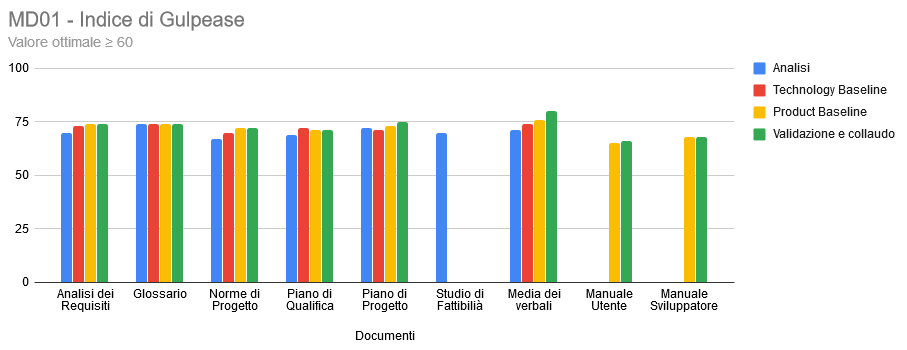
\includegraphics[scale=0.7]{./img/MD01_gulpease.png}
\caption{Grafico relativo ai dati di MD01 - Indice di Gulpease}
\end{figure}

\paragraph{Esiti MD02 - Indice Fog} \mbox{} \\
\begin{longtable}{c c c c c c}
\rowcolor{white}\caption{Esiti MD02 - Indice Fog} \\
		\rowcolor{redafk}
\textcolor{white}{\textbf{Attività}} &
\textcolor{white}{\textbf{An}} &
\textcolor{white}{\textbf{TB}} &
\textcolor{white}{\textbf{PB}} &
\textcolor{white}{\textbf{VC}} &
\textcolor{white}{\textbf{Riscontro}}  \\
		\endfirsthead
		\rowcolor{white}\caption[]{(continua)} \\
		\rowcolor{redafk}
\textcolor{white}{\textbf{Attività}} &
\textcolor{white}{\textbf{An}} &
\textcolor{white}{\textbf{TB}} &
\textcolor{white}{\textbf{PB}} &
\textcolor{white}{\textbf{VC}} &
\textcolor{white}{\textbf{Riscontro}}  \\
		\endhead
\textit{Analisi dei Requisiti} & 18 & 17 & 17 & 17 & Accettabile\\
\textit{Glossario} & 15 & 15 & 13 & 13 & Accettabile \\
\textit{Norme di Progetto} & 20 & 18 & 16 & 16 & Accettabile\\
\textit{Piano di Progetto} & 18 & 20 & 20 & 19 & Accettabile\\
\textit{Piano di Qualifica} & 20 & 20 & 20 & 20 & Accettabile\\
\textit{Studio di Fattibilità} & 14 & - & - & - & Accettabile\\
\textit{Media Verbali} & 8 & 6 & 6 & 6 & Ottimale\\
\textit{Manuale Utente} & - & - & 16 & 15 & Accettabile \\
\textit{Manuale Sviluppatore} & - & - & 19 & 19 & Accettabile\\
\end{longtable}

\begin{figure}[H]
\centering
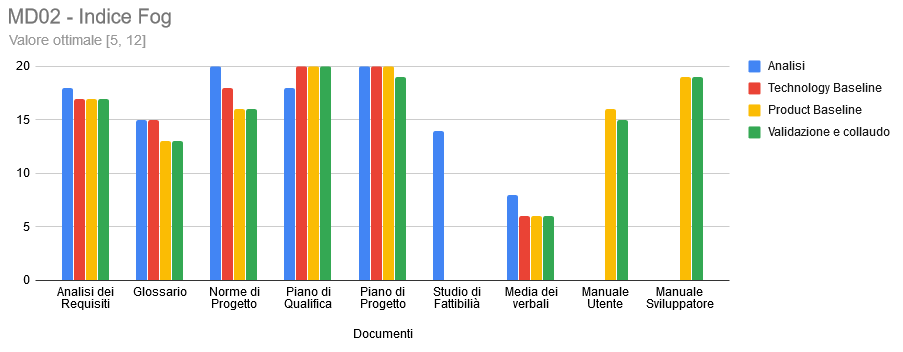
\includegraphics[scale=0.7]{./img/MD02_fog.png}
\caption{Grafico relativo ai dati di MD02 - Indice Fog}
\end{figure}

\subsection{Analisi metriche di qualità generale del prodotto}
\subsubsection{Esiti MG01 - Percentuale di metriche soddisfatte}
\begin{longtable}{c c c c c}
\rowcolor{white}\caption{Esiti MG01 - PMS}\\
		\rowcolor{redafk}
		\textcolor{white}{\textbf{Periodo}} &
\textcolor{white}{\textbf{Metriche soddisfatte}} & \textcolor{white}{\textbf{Totale}} & 
\textcolor{white}{\textbf{Percentuale}} & \textcolor{white}{\textbf{Esito}}\\
		\endfirsthead
		\rowcolor{white}\caption[]{(continua)} \\
		\rowcolor{redafk}
		\textcolor{white}{\textbf{Periodo}} &
\textcolor{white}{\textbf{Metriche Soddisfatte}} & \textcolor{white}{\textbf{Totale}} & 
\textcolor{white}{\textbf{Percentuale}} & \textcolor{white}{\textbf{Esito}}\\
		\endhead
		PB & 18 & 19 & 94.7\% & Accettabile\\
		VC & 19 & 19 & 100\% & Ottimale\\
\end{longtable}

\begin{figure}[H]
\centering
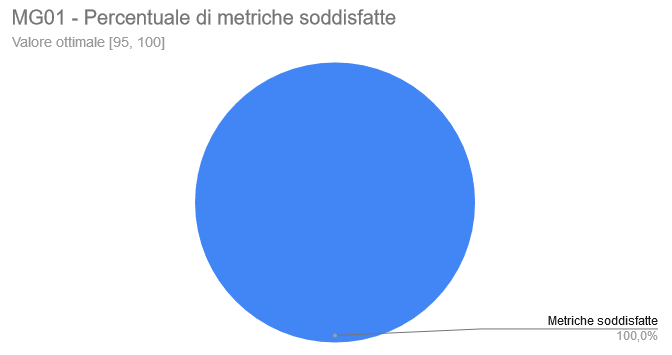
\includegraphics[scale=0.7]{./img/MG01.png}
\caption{Grafico relativo ai dati di MG01 - Percentuale di metriche soddisfatte}
\end{figure}

\subsubsection{Esiti MG02 - Percentuale di requisiti obbligatori soddisfatti}
\begin{longtable}{C{3cm} C{3cm} L{5.5cm} C{3cm}}
\rowcolor{white}\caption{Tabella del soddisfacimento dei requisiti obbligatori}\\
		\rowcolor{redafk}
\textcolor{white}{\textbf{Codice}} & \textcolor{white}{\textbf{Esito}}\\
		\endfirsthead
		\rowcolor{white}\caption[]{(continua)} \\
		\rowcolor{redafk}
\textcolor{white}{\textbf{Codice}} & \textcolor{white}{\textbf{Esito}}\\
		\endhead
		
Re1F1 	& Soddisfatto\\
Re1F1.1 & Soddisfatto\\
Re1F1.2 & Soddisfatto\\
Re1F1.3 & Soddisfatto\\
Re1F1.4 & Soddisfatto\\
Re1F1.6 & Soddisfatto\\
Re1F1.7 & Soddisfatto\\
Re1F2 	& Soddisfatto\\
Re1F2.1 & Soddisfatto\\
Re1F2.2 & Soddisfatto\\
Re1F2.4 & Soddisfatto\\
Re1F3 	& Soddisfatto\\
Re1F3.1 & Soddisfatto\\
Re1F3.2 & Soddisfatto\\
Re1F3.4 & Soddisfatto\\
Re1F3.5 & Soddisfatto\\
Re1F3.6 & Soddisfatto\\
Re1F4 	& Soddisfatto\\
Re1F5 	& Soddisfatto\\
Re1F5.1 & Soddisfatto\\
Re1F5.2 & Soddisfatto\\
Re1F5.3 & Soddisfatto\\
Re1F5.5 & Soddisfatto\\
Re1F6 	& Soddisfatto\\
Re1F6.1 & Soddisfatto\\
Re1F6.2 & Soddisfatto\\
Re1F6.3 & Soddisfatto\\
Re1F6.5 & Soddisfatto\\
Re1F7 	& Soddisfatto\\
Re1F7.1 & Soddisfatto\\
Re1F7.2 & Soddisfatto\\
Re1F8 	& Soddisfatto\\
Re1F8.1 & Soddisfatto\\
Re1F8.2 & Soddisfatto\\
Re1F8.3 & Soddisfatto\\
Re1F8.5 & Soddisfatto\\
Re1F9 	& Soddisfatto\\
Re1F9.1 & Soddisfatto\\
Re1F10 	& Soddisfatto\\
Re1F10.1& Soddisfatto\\
Re1F11 	& Soddisfatto\\
Re1F12 	& Soddisfatto\\
Re1F13 	& Soddisfatto\\
Re1F14 	& Soddisfatto\\
Re1F16 	& Soddisfatto\\
Re1F17 	& Soddisfatto\\
Re1F18 	& Soddisfatto\\
Re1Q1 	& Soddisfatto\\
Re1Q2 	& Soddisfatto\\
Re1Q2.1 & Soddisfatto\\
Re1Q3 	& Soddisfatto\\
Re1Q4 	& Soddisfatto\\
Re1V1 	& Soddisfatto\\
Re1V1.1 & Soddisfatto\\
Re1V1.2 & Soddisfatto\\
Re1V1.3 & Soddisfatto\\
Re1V1.4 & Soddisfatto\\
Re1V2 	& Soddisfatto\\
Re1V3 	& Soddisfatto\\
Re1V4 	& Soddisfatto\\
Re1V5 	& Soddisfatto\\
\end{longtable}

\begin{longtable}{c c c c c}
\rowcolor{white}\caption{Esiti MG02 - PROS}\\
		\rowcolor{redafk}
		\textcolor{white}{\textbf{Periodo}} &
\textcolor{white}{\textbf{Requisiti Obbligatori Soddisfatti}} & \textcolor{white}{\textbf{Totale}} & 
\textcolor{white}{\textbf{Percentuale}} & \textcolor{white}{\textbf{Esito}}\\
		\endfirsthead
		\rowcolor{white}\caption[]{(continua)} \\
		\rowcolor{redafk}
		\textcolor{white}{\textbf{Periodo}} &
\textcolor{white}{\textbf{Requisiti Obbligatori Soddisfatti}} & \textcolor{white}{\textbf{Totale}} & 
\textcolor{white}{\textbf{Percentuale}} & \textcolor{white}{\textbf{Esito}}\\
		\endhead
		PB & 48 & 61 & 79,2\% & Accettabile \\
		VC & 61 & 61 & 100\% & Ottimale \\
\end{longtable}

\begin{figure}[H]
\centering
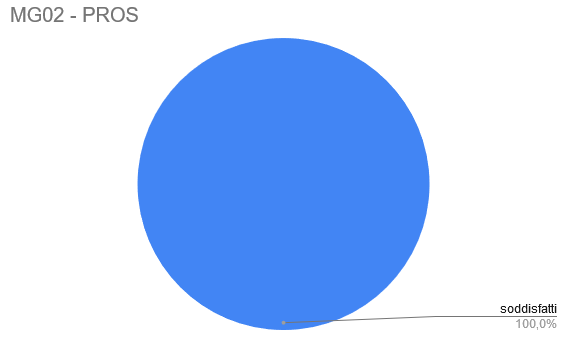
\includegraphics[scale=0.7]{./img/MG02.png}
\caption{Grafico relativo ai dati di MG02 - PROS}
\end{figure}

\subsubsection{Esiti MG03 - Percentuale di requisiti desiderabili soddisfatti}
\begin{longtable}{C{3cm} C{3cm} L{5.5cm} C{3cm}}
\rowcolor{white}\caption{Tabella del soddisfacimento dei requisiti desiderabili}\\
		\rowcolor{redafk}
\textcolor{white}{\textbf{Codice}} & \textcolor{white}{\textbf{Esito}}\\
		\endfirsthead
		\rowcolor{white}\caption[]{(continua)} \\
		\rowcolor{redafk}
\textcolor{white}{\textbf{Codice}} & \textcolor{white}{\textbf{Esito}}\\
		\endhead
		
Re2F1.5 & Soddisfatto\\
Re2F2.3 & Soddisfatto\\
Re3F3.4 & Non soddisfatto\\
Re2F5.4 & Soddisfatto\\ 
Re2F6.4 & Soddisfatto\\
Re2F7.2 & Soddisfatto\\
Re2F8.4 & Soddisfatto\\
Re2F8.6 & Soddisfatto\\
Re2F9.2 & Soddisfatto\\
Re3F10.2 & Non soddisfatto\\
Re3F15 & Non soddisfatto\\
Re2Q5 	& Soddisfatto\\
Re2Q6 	& Soddisfatto\\
Re2Q7 	& Soddisfatto\\
\end{longtable}

\begin{longtable}{c c c c c}
\rowcolor{white}\caption{Esiti MG03 - PRDS}\\
		\rowcolor{redafk}
		\textcolor{white}{\textbf{Periodo}} &
\textcolor{white}{\textbf{Requisiti Desiderabili Soddisfatti}} & \textcolor{white}{\textbf{Totale}} & 
\textcolor{white}{\textbf{Percentuale}} & \textcolor{white}{\textbf{Esito}}\\
		\endfirsthead
		\rowcolor{white}\caption[]{(continua)} \\
		\rowcolor{redafk}
		\textcolor{white}{\textbf{Periodo}} &
\textcolor{white}{\textbf{Requisiti Desiderabili Soddisfatti}} & \textcolor{white}{\textbf{Totale}} & 
\textcolor{white}{\textbf{Percentuale}} & \textcolor{white}{\textbf{Esito}}\\
		\endhead
		PB & 9 & 14 & 61,5\% & Accettabile \\
		VC & 11 & 14 & 78.6\% & Accettabile \\
\end{longtable}

\begin{figure}[H]
\centering
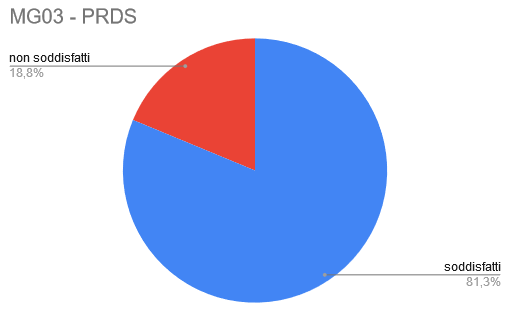
\includegraphics[scale=0.7]{./img/MG03.png}
\caption{Grafico relativo ai dati di MG03 - PRDS}
\end{figure}

\subsection{Analisi metriche dei processi}
\subsubsection{Esiti MP01 - Schedule Variance} 
\begin{longtable}{c c c c c c}
\rowcolor{white}\caption{Esiti MP01 - Schedule Variance} \\
		\rowcolor{redafk}
\textcolor{white}{\textbf{Attività}} &
\textcolor{white}{\textbf{An}} &
\textcolor{white}{\textbf{TB}} &
\textcolor{white}{\textbf{PB}} &
\textcolor{white}{\textbf{VC}} &
\textcolor{white}{\textbf{Riscontro}} \\
		\endfirsthead
		\rowcolor{white}\caption[]{(continua)} \\
		\rowcolor{redafk}
\textcolor{white}{\textbf{Attività}} &
\textcolor{white}{\textbf{An}} &
\textcolor{white}{\textbf{TB}} &
\textcolor{white}{\textbf{PB}} &
\textcolor{white}{\textbf{VC}} &
\textcolor{white}{\textbf{Riscontro}} \\
		\endhead
\textit{Analisi dei Requisiti} & 
1 &
1 &
0 &
0 &
Ottimale \\
\textit{Glossario} & 
0 &
0 &
0 &
0 &
Ottimale \\
\textit{Norme di Progetto} & 
0 &
1 &
0 &
0 &
Ottimale \\
\textit{Piano di Qualifica} & 
1 &
-2 &
4 &
2 &
Accettabile \\
\textit{Piano di Progetto} & 
1 &
0 &
0 &
0 &
Ottimale \\
\textit{Studio di Fattibilià} & 
0 &
- &
- &
- &
Ottimale \\
\textit{Manuale Utente} &
- &
- &
0 &
0 &
Ottimale \\
\textit{Manuale Sviluppatore} &
- &
- &
2 &
1 &
Accettabile \\
\end{longtable}

\begin{figure}[H]
\centering
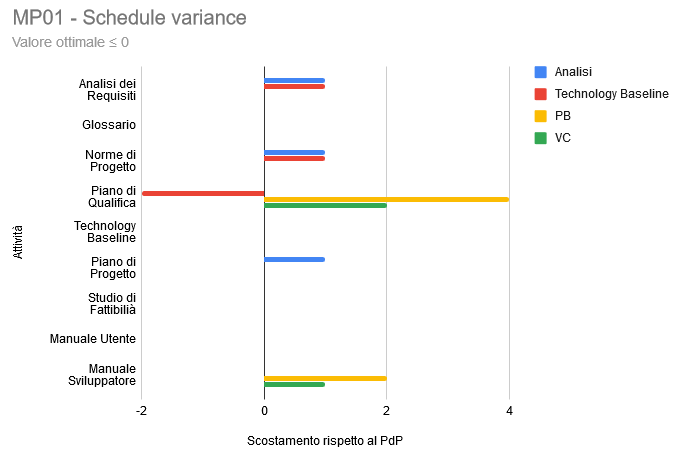
\includegraphics[scale=0.7]{./img/MP01_schedule_variance.png}
\caption{Grafico relativo ai dati di MP01 - Schedule Variance}
\end{figure}
\pagebreak
\subsubsection{Esiti MP02 - Budget Variance}
\begin{longtable}{c c c c c}
\rowcolor{white}\caption{Esiti MP02 - Budget Variance} \\
		\rowcolor{redafk}
\textcolor{white}{\textbf{An}} &
\textcolor{white}{\textbf{TB}} &
\textcolor{white}{\textbf{PB}} &
\textcolor{white}{\textbf{VC}} &
\textcolor{white}{\textbf{Riscontro}} \\
-8,66$\%$ &
-1,19$\%$ &
+0,94$\%$ &
+2,65$\%$ &
Ottimale \\
\end{longtable}

\begin{figure}[H]
\centering
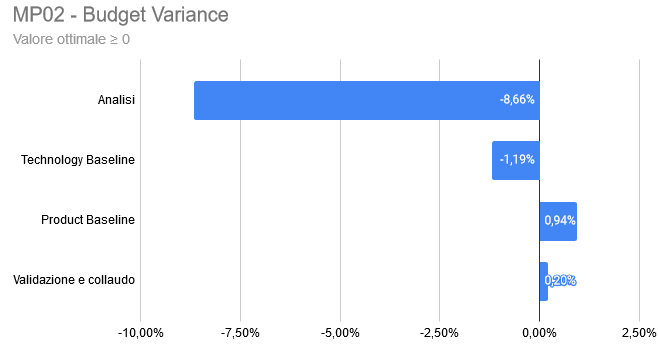
\includegraphics[scale=0.7]{./img/MP02_budget_variance.png}
\caption{Grafico relativo ai dati di MP02 - Budget Variance}
\end{figure}

\subsubsection{Esiti MP03 - Produttività} 
\begin{longtable}{c c c c c c}
\rowcolor{white}\caption{Esiti MP03 - Produttività} \\
		\rowcolor{redafk}
\textcolor{white}{\textbf{Membro}} &
\textcolor{white}{\textbf{An}} &
\textcolor{white}{\textbf{TB}} &
\textcolor{white}{\textbf{PB}} &
\textcolor{white}{\textbf{VC}} &
\textcolor{white}{\textbf{Riscontro}} \\
		\endfirsthead
		\rowcolor{white}\caption[]{(continua)} \\
		\rowcolor{redafk}
		\textcolor{white}{\textbf{Membro}} &
\textcolor{white}{\textbf{An}} &
\textcolor{white}{\textbf{TB}} &
\textcolor{white}{\textbf{PB}} &
\textcolor{white}{\textbf{VC}} &
\textcolor{white}{\textbf{Riscontro}} \\
		\endhead
Simone Federico Bergamin & 0 & 78 & 188 & - & Ottimale\\
Alessandro Canesso & 0 & 139 & 150 & - & Ottimale \\
Victor Dutca & 0 & 108 & 183 & - & Ottimale \\
Fouad Farid & 0 & 109 & 320 & - & Ottimale \\
Simone Meneghin & 0 & 93 & 292 & - & Ottimale\\
Olivier Utshudi & 0 & 93 & 245 & - & Ottimale\\
Davide Zilio & 0 & 93 & 204 & - & Ottimale\\
\end{longtable}

\begin{figure}[H]
\centering
\includegraphics[scale=0.7]{./img/MP03_produttività.png}
\caption{Grafico relativo ai dati di MP03 - Produttività}
\end{figure}

\subsection{Analisi metriche del software}
\subsubsection{Esiti MS01 - LOC per metodo}
\begin{longtable}{c c c c c}
\rowcolor{white}\caption{Esiti MS01 - LOC per metodo} \\
	\rowcolor{redafk}
	\textcolor{white}{\textbf{Periodo}} &
	\textcolor{white}{\textbf{Tot\_LOC}} &
	\textcolor{white}{\textbf{\#Metodi}} &
\textcolor{white}{\textbf{Rapporto}} &
\textcolor{white}{\textbf{Esito}} \\
	\endfirsthead
		\rowcolor{white}\caption[]{(continua)} \\
		\rowcolor{redafk}
	\textcolor{white}{\textbf{Periodo}} &
	\textcolor{white}{\textbf{Tot\_LOC}} &
	\textcolor{white}{\textbf{\#Metodi}} &
\textcolor{white}{\textbf{Rapporto}} &
\textcolor{white}{\textbf{Esito}} \\
	\endhead
	TB & 713 & 60 & 11.88 & Accettabile\\	
	PB & 2270 & 114 & 19.91 & Accettabile \\
\end{longtable}

\begin{figure}[H]
\centering
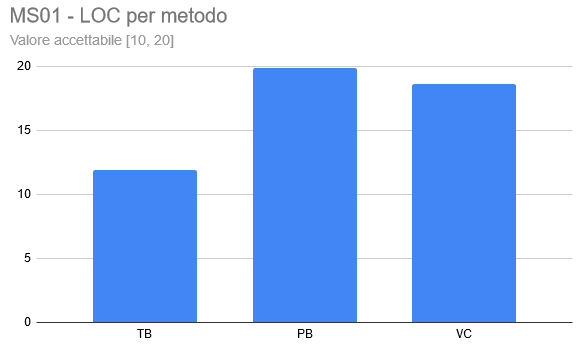
\includegraphics[scale=0.7]{./img/MS01.png}
\caption{Grafico relativo ai dati di MS01 - LOC per metodo}
\end{figure}

\subsubsection{Esiti MS02 - Numero di metodi}
\begin{longtable}{c C{3cm} C{2cm} C{2cm} C{2cm}}
\rowcolor{white}\caption{Esiti MS02 - Numero di metodi} \\
	\rowcolor{redafk}
	\textcolor{white}{\textbf{Periodo}} &
	\textcolor{white}{\textbf{Tot\_metodi}} &
	\textcolor{white}{\textbf{\#Classi}} &
\textcolor{white}{\textbf{Rapporto}} &
\textcolor{white}{\textbf{Esito}} \\
	\endfirsthead
		\rowcolor{white}\caption[]{(continua)} \\
		\rowcolor{redafk}
		\textcolor{white}{\textbf{Periodo}} &
	\textcolor{white}{\textbf{Tot\_metodi}} &
	\textcolor{white}{\textbf{\#Classi}} &
\textcolor{white}{\textbf{Rapporto}} &
\textcolor{white}{\textbf{Esito}} \\
	\endhead
	TB & 43 & 17 & 2.53 & Ottimale \\
	PB & 117 & 34 & 3.44 & Ottimale \\
\end{longtable}

\begin{figure}[H]
\centering
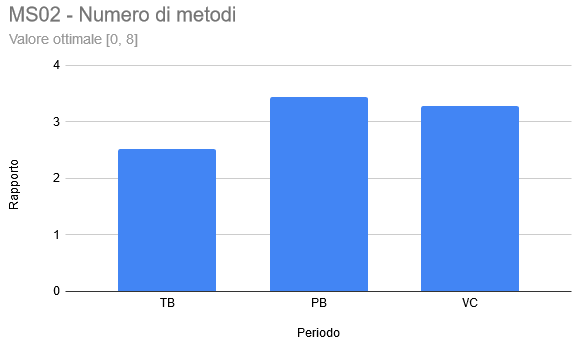
\includegraphics[scale=0.7]{./img/MS02.png}
\caption{Grafico relativo ai dati di MS02 - Numero di metodi medio per classe}
\end{figure}

\subsubsection{Esiti MS03 - Numero di parametri}
\begin{longtable}{c C{2cm} C{3cm} C{2cm} C{2.5cm}}
\rowcolor{white}\caption{Esiti MS03 - Numero di parametri} \\
	\rowcolor{redafk}
	\textcolor{white}{\textbf{Periodo}} &
	\textcolor{white}{\textbf{\#metodi}} &
	\textcolor{white}{\textbf{\#parametri}} &
\textcolor{white}{\textbf{Rapporto}} &
\textcolor{white}{\textbf{Esito}} \\
	\endfirsthead
		\rowcolor{white}\caption[]{(continua)} \\
		\rowcolor{redafk}
		\textcolor{white}{\textbf{Periodo}} &
	\textcolor{white}{\textbf{\#metodi}} &
	\textcolor{white}{\textbf{\#parametri\_passati}} &
\textcolor{white}{\textbf{Rapporto}} &
\textcolor{white}{\textbf{Esito}} \\
	\endhead
	TB & 43 & 11 & 3.91 & Accettabile \\
	PB & 117 & 46 & 2.54 & Ottimale \\
\end{longtable}

\begin{figure}[H]
\centering
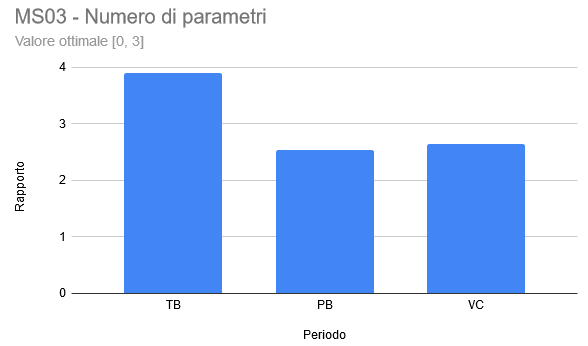
\includegraphics[scale=0.7]{./img/MS03.png}
\caption{Grafico relativo ai dati di MS03 - Numero di parametri medio per metodo}
\end{figure}

\subsubsection{Esiti MS04 - Commenti per LOC}
\begin{longtable}{c c c c c}
\rowcolor{white}\caption{Esiti MS04 - Commenti per LOC} \\
	\rowcolor{redafk}
	\textcolor{white}{\textbf{Periodo}} &
	\textcolor{white}{\textbf{Tot\_LOC}} &
	\textcolor{white}{\textbf{Tot\_commenti}} &
\textcolor{white}{\textbf{Rapporto}} &
\textcolor{white}{\textbf{Esito}} \\
	\endfirsthead
		\rowcolor{white}\caption[]{(continua)} \\
		\rowcolor{redafk}
		\textcolor{white}{\textbf{Periodo}} &
		\textcolor{white}{\textbf{Tot\_LOC}} &
\textcolor{white}{\textbf{Tot\_commenti}} &
\textcolor{white}{\textbf{Rapporto}} & 
\textcolor{white}{\textbf{Esito}} \\
	\endhead
	TB & 713 & 7 & 0.01 & Non accettabile\\	
	PB & 2270 & 135 & 0.06 & Accettabile
\end{longtable}

\begin{figure}[H]
\centering
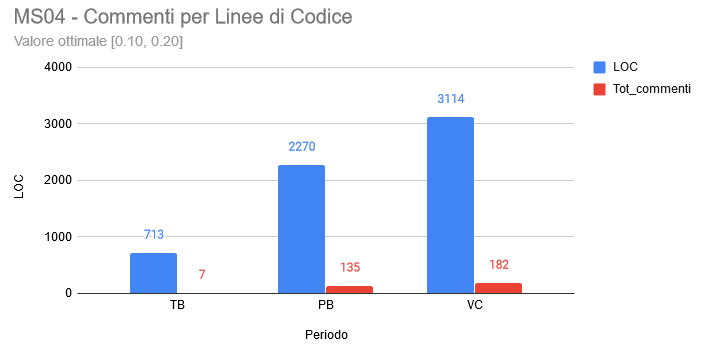
\includegraphics[scale=0.7]{./img/MS04.png}
\caption{Grafico relativo ai dati di MS04 - Commenti per LOC}
\end{figure}

\subsubsection{Esiti MS05-MS06 - Fan In/Fan Out}
\begin{longtable}{c c c}
\rowcolor{white}\caption{Esiti MS05-MS06 - Fan In/Fan Out} \\
	\rowcolor{redafk}
	\textcolor{white}{\textbf{Periodo}} &
	\textcolor{white}{\textbf{Fan In}} &
	\textcolor{white}{\textbf{Fan Out}}\\
	\endfirsthead
		\rowcolor{white}\caption[]{(continua)} \\
		\rowcolor{redafk}
		\textcolor{white}{\textbf{Periodo}} &
	\textcolor{white}{\textbf{Fan In}} &
	\textcolor{white}{\textbf{Fan Out}}\\
	\endhead
	TB & 31 & 26\\	
	PB & 43 & 33\\	
\end{longtable}

\begin{figure}[H]
\centering
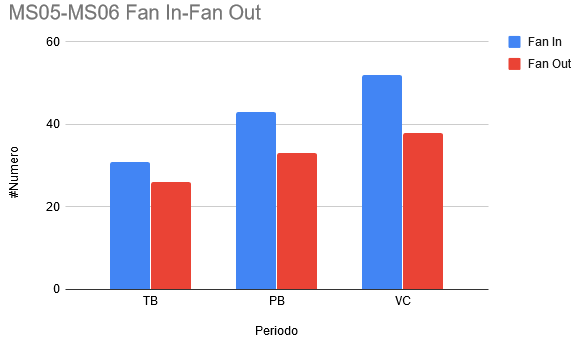
\includegraphics[scale=0.7]{./img/MS05-MS06.png}
\caption{Grafico relativo ai dati di MS05-MS06 - Fan In/Fan Out}
\end{figure}

\pagebreak
\subsection{Analisi metriche dei test}
\subsubsection{Esiti MS07 - Code Coverage}
\begin{longtable}{c c c}
\rowcolor{white}\caption{Esiti MS07 - Code Coverage} \\
	\rowcolor{redafk}
\textcolor{white}{\textbf{Periodo}} & 
\textcolor{white}{\textbf{Percentuale}} & 
\textcolor{white}{\textbf{Riscontro}} \\
	\endfirsthead
		\rowcolor{white}\caption[]{(continua)} \\
		\rowcolor{redafk}
\textcolor{white}{\textbf{Periodo}} & 
\textcolor{white}{\textbf{Percentuale}} & 
\textcolor{white}{\textbf{Riscontro}} \\
	\endhead
	TB & 29\% & Non accettabile\\
	PB & 73\% & Accettabile\\
	VC & 96\% & Ottimale\\
\end{longtable}

\begin{figure}[H]
\centering
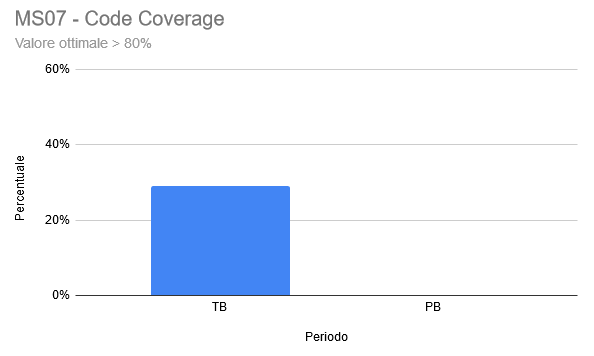
\includegraphics[scale=0.7]{./img/MS07.png}
\caption{Grafico relativo ai dati di MS07 - Code Coverage}
\end{figure}

\subsubsection{Esiti MS08/MS09 - Passed/Failed Test Case Percentage}
\begin{longtable}{c C{3cm} C{3cm} C{3cm}}
\rowcolor{white}\caption{Esiti MS08/MS09 - PTCP-FTCP} \\
	\rowcolor{redafk}
	\textcolor{white}{\textbf{Periodo}} &
\textcolor{white}{\textbf{Metrica}} &
\textcolor{white}{\textbf{Percentuale}} & 
\textcolor{white}{\textbf{Riscontro}} \\
	\endfirsthead
		\rowcolor{white}\caption[]{(continua)} \\
		\rowcolor{redafk}
		\textcolor{white}{\textbf{Periodo}} &
\textcolor{white}{\textbf{Metrica}} &
\textcolor{white}{\textbf{Percentuale}} & 
\textcolor{white}{\textbf{Riscontro}} \\
	\endhead
	TB & PTCP \newline FTCP & 100\% \newline 0\% & Ottimale \newline Ottimale\\
	PB & PTCP \newline FTCP & 100\% \newline 0\% & Ottimale \newline Ottimale\\
	VC & PTCP \newline FTCP & 100\% \newline 0\% & Ottimale \newline Ottimale\\
\end{longtable}

\begin{figure}[H]
\centering
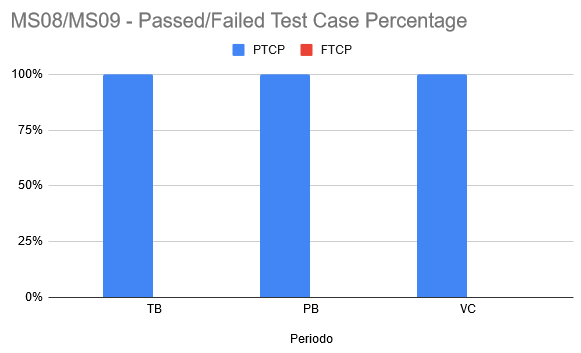
\includegraphics[scale=0.7]{./img/MS08-MS09.png}
\caption{Grafico relativo ai dati di MS08-MS09 PTCP-FTCP}
\end{figure}

\subsubsection{Esiti MS10 - Requisiti obbligatori implementati}
\begin{longtable}{c c c}
\rowcolor{white}\caption{Esito MS10 - ROI} \\
	\rowcolor{redafk}
\textcolor{white}{\textbf{Attività}} &
\textcolor{white}{\textbf{Percentuale}} & 
\textcolor{white}{\textbf{Riscontro}} \\
	\endfirsthead
\textcolor{white}{\textbf{Attività}} &
\textcolor{white}{\textbf{Percentuale}} & 
\textcolor{white}{\textbf{Riscontro}} \\
	\endhead
	TB & 41,6\% & Non accettabile\\
	PB & 79,2\% & Accettabile\\
	VC & 100\% & Ottimale\\
\end{longtable}

\begin{figure}[H]
\centering
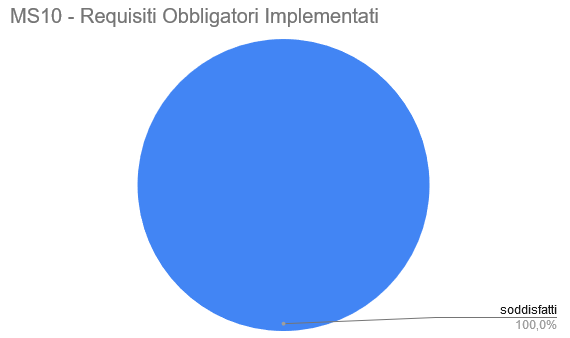
\includegraphics[scale=0.7]{./img/MS10.png}
\caption{Grafico relativo ai dati di MS10 - ROI}
\end{figure}


\subsubsection{Esiti MS11 - Requisiti desiderabili implementati}
\begin{longtable}{c c c}
\rowcolor{white}\caption{Esito MS11 - RDI} \\
	\rowcolor{redafk}
\textcolor{white}{\textbf{Attività}} &
\textcolor{white}{\textbf{Percentuale}} & 
\textcolor{white}{\textbf{Riscontro}} \\
	\endfirsthead
\textcolor{white}{\textbf{Attività}} &
\textcolor{white}{\textbf{Percentuale}} & 
\textcolor{white}{\textbf{Riscontro}} \\
	\endhead
	TB & 29,3\% & Non accettabile \\
	PB & 61,5\% & Accettabile \\
	VC & 78.6\% & Accettabile \\
\end{longtable}

\begin{figure}[H]
\centering
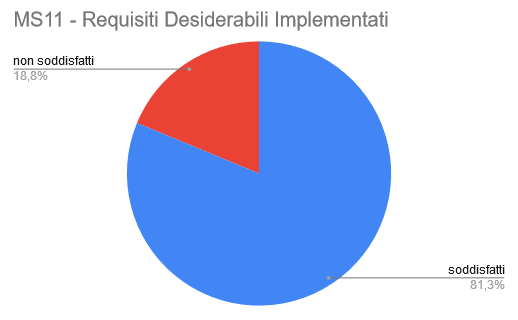
\includegraphics[scale=0.7]{./img/MS11.png}
\caption{Grafico relativo ai dati di MS11 - RDI}
\end{figure}

